\documentclass[a4paper, 11pt]{article}
\usepackage[left=2cm, top=3cm, text={17cm,24cm}]{geometry}
\usepackage[czech]{babel}
\usepackage[utf8]{inputenc}
\usepackage{times}
\usepackage{multirow}
\usepackage[ruled,czech,linesnumbered,longend,noline]{algorithm2e}
\usepackage{algorithmic}
\usepackage{picture}
\usepackage{graphics}
\usepackage{epstopdf}
\usepackage{pdflscape}
\newcommand{\myuv}[1]{\quotedblbase #1\textquotedblleft}

\begin{document}
\begin{titlepage}
\begin{center}
\textsc{\Huge Vysoké učení technické v Brně\\ \medskip
\huge Fakulta informačních technologií}\\
\vspace{\stretch{0.382}}
\LARGE Typografie a publikování\,--\,3. projekt\\
\Huge Tabulky a obrázky\\
\vspace{\stretch{0.618}}
\Large \today \hfill         Tomáš Zubrik \newpage
\end{center}
\end{titlepage}
\newpage

\section{Úvodní strana}
Název práce umístěte do zlatého řezu a~nezapomeňte uvést dnešní datum a~vaše jméno a~příjmení.

\section{Tabulky}
Pro sázení tabulek můžeme použít buď prostředí\texttt{ tabbing }nebo prostředí\texttt{ tabular}.

\subsection{Prostředí\texttt{ tabbing}}
Při použití\texttt{ tabbing }vypadá tabulka následovně:

%----------------------------Fruit Table----------------------------%
\begin{tabbing}
\verb|\pushtabs| \qquad \= \textbf{Cena} \quad\= \kill
\textbf{Ovoce} \> \textbf{Cena} \> \textbf{Množství} \\
Jablka\> 25,90\> 3 kg\\
Hrušky\> 27,40\> 2,5 kg\\
Vodní melouny\> 35,-- \> 1 kus\\
\end{tabbing}

\noindent Toto prostředí se dá také použít pro sázení algoritmů, ovšem vhodnější je použít 
prostředí\texttt{ algorithm }nebo \texttt{ algorithm2e } (viz sekce \ref{algorithm}).

\subsection{Prostředí\texttt{ tabular}}
Další možností, jak vytvořit tabulku, je použít prostředí\texttt{ tabular}. Tabulky pak budou
vypadat takto\footnote{Kdyby byl problém s\texttt{ cline, }zkuste se podívat teba sem:
http://www.abclinuxu.cz/tex/poradna/show/325037.}:
\bigskip

\begin{table}[h] 
\begin{center}
\catcode`\-=12 
%----------------------------Currency Table----------------------------%
\begin{tabular}{|l|r|r|} 
\hline
& \multicolumn{2}{|c|}{\textbf{Cena}}\\ \cline{2-3}
\textbf{Měna} & \textbf{nákup} & \textbf{prodej}\\ \hline
EUR & 27,02 & 27,20\\
GBP & 31,08 & 31,80\\
USD & 25,15 & 25,51\\
\hline
\end{tabular}
\caption{Tabulka kurzů k~dnešnímu dni}
\label{course}
\end{center}
\end{table}

\begin{table}[h] 
\begin{center}
\catcode`\-=12 
%----------------------------1st Table----------------------------% 
\begin{tabular}{|c|c|} 
\hline
$A$ & $\neg A$\\ \hline
$\textbf{P}$ & $N$\\ \hline
$\textbf{O}$ & $O$\\ \hline
$\textbf{X}$ & $X$\\ \hline
$\textbf{N}$ & $P$\\
\hline
\end{tabular}
%----------------------------2nd Table----------------------------%
\begin{tabular}{|c|c|c|c|c|c|} \hline
\multicolumn{2}{|l|}{\multirow{2}{*}{$A \wedge B$}} & \multicolumn{4}{c|}{$B$}  \\ \cline{3-6} 
\multicolumn{2}{|c|}{} & \textbf{P} & \textbf{O} & \textbf{X} & \textbf{N} \\ \hline
\multirow{4}{*}{$A$} & \textbf{P} & P & O & X & N \\ \cline{2-6} 
 & \textbf{O} & O & O & N & N \\ \cline{2-6}  
 & \textbf{X} & X & N & X & N \\ \cline{2-6} 
 & \textbf{N} & N & N & N & N \\ \hline 
\end{tabular}
%----------------------------3rd Table----------------------------%
\begin{tabular}{|c|c|c|c|c|c|} \hline
\multicolumn{2}{|l|}{\multirow{2}{*}{$A \vee B$}} & \multicolumn{4}{c|}{$B$}  \\ \cline{3-6} 
\multicolumn{2}{|c|}{} & \textbf{P} & \textbf{O} & \textbf{X} & \textbf{N} \\ \hline
\multirow{4}{*}{$A$} & \textbf{P} & P & P & P & P \\ \cline{2-6} 
 & \textbf{O} & P & O & P & O \\ \cline{2-6}  
 & \textbf{X} & P & P & X & X \\ \cline{2-6} 
 & \textbf{N} & P & O & X & N \\ \hline 
\end{tabular}
%----------------------------4th Table----------------------------%
\begin{tabular}{|c|c|c|c|c|c|} \hline
\multicolumn{2}{|l|}{\multirow{2}{*}{$A \rightarrow B$}} & \multicolumn{4}{c|}{$B$}  \\ \cline{3-6} 
\multicolumn{2}{|c|}{} & \textbf{P} & \textbf{O} & \textbf{X} & \textbf{N} \\ \hline
\multirow{4}{*}{$A$} & \textbf{P} & P & O & X & N \\ \cline{2-6} 
 & \textbf{O} & P & O & P & O \\ \cline{2-6}  
 & \textbf{X} & P & P & X & X \\ \cline{2-6} 
 & \textbf{N} & P & P & P & P \\ \hline 
\end{tabular}
\caption{Protože Kleeneho trojhodnotová logika už je \myuv{zastaralá}, uvádíme si zde příklad čtyřhodnotové
logiky}
\label{logic}
\end{center}
\end{table}
\section{Algoritmy} \label{algorithm}
Pokud budeme chtít vysázet algoritmus, můžeme použít prostředí\texttt{ algorithm\footnote{Pro nápovědu, jak zacházet s prostředím\texttt{ algorithm, }můžeme zkusit tuhle 
stránku:\\http://ftp.cstug.cz/pub/tex/CTAN/macros/latex/contrib/algorithms/algorithms.pdf.} } 
nebo\texttt{ algorithm2e\footnote{Pro\texttt{ algorithm2e }zase tuhle: http://ftp.cstug.cz/pub/tex/CTAN/macros/latex/contrib/algorithm2e/doc/algorithm2e.pdf.}}.
Příklad použití prostředí\texttt{ algorithm2e }viz Algoritmus \ref{algorithm-src}. 
\bigskip
%----------------------------Algorithm----------------------------%
\begin{algorithm}[h]
\label{algorithm-src}
\caption{\textsc{Fast}SLAM}
\SetKwInput{Input}{Input }
\SetKwInOut{Output}{Output }
\SetInd{1em}{1em}
\SetNlSkip{-1.20em}
\SetNlSty{}{}{:}
\Input{($X_{t-1}, u_t, z_t$)}
\Output{$X_t$}
\BlankLine
\Indp \Indp
$\overline{X_t} = X_t = 0$\\
\For{$k = 1 \textnormal{ to } M$}
{
	$x^{[k]}_{t} = sample\_motion\_mode(u_t ,x^{[k]}_{t-1})$\\
	$\omega^{[k]}_{t} = measurement\_model(z_t ,x^{[k]}_{t}, m_{t-1})$\\
	$m^{[k]}_{t} = updated\_occupancy\_grid(z_t ,x^{[k]}_{t}, m_{t-1}^{[k]})$\\
	$\overline{X_t} = \overline{X_t} + \langle x^{[m]}_{x}, \omega^{[m]}_{t} \rangle$\\
}
\For{$k = 1 \textnormal{ to } M$}
{
	$\textnormal{draw } i \textnormal{ with probability} \approx \omega^{[i]}_{t}$\\
	$\textnormal{add } \langle x^{[k]}_{x}, m^{[k]}_{t} \rangle \textnormal{ to } X_t$\\
}
\Return{$X_t$}   
\end{algorithm}

\section{Obrázky}
Do našich článků můžeme samozřejmě vkládat obrázky. Pokud je obrázkem fotografie,
můžeme klidně použít bitmapový soubor. Pokud by to ale mělo být nějaké schéma nebo
něco podobného, je dobrým zvykem takovýto obrázek vytvořit vektorově.
%----------------------------Ethiopan Mirror Picture----------------------------%
\begin{figure}[h]
\center{
\scalebox{0.4}{
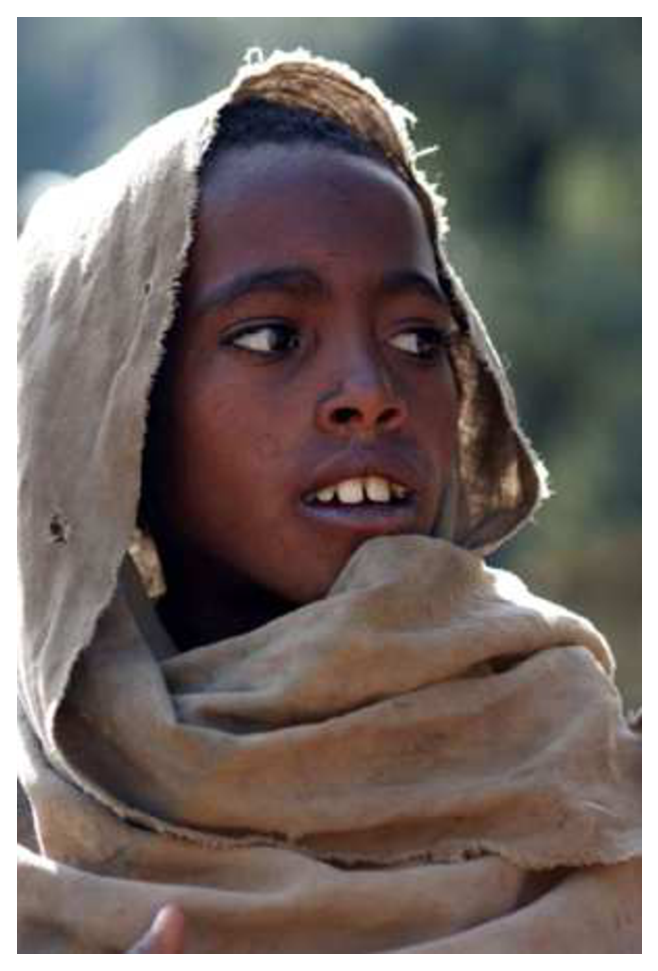
\includegraphics{etiopan.eps}
\reflectbox{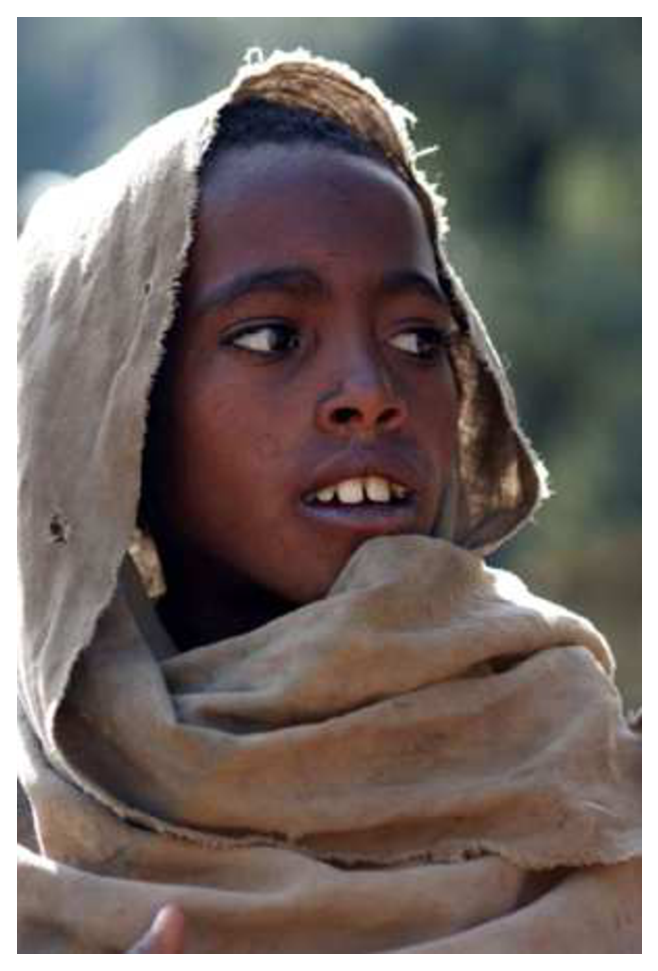
\includegraphics{etiopan.eps}}}}
\caption{Malý etiopánek a jeho bratříček}
\label{ethiopan}
\end{figure}
\newpage

%----------------------------Vector Picture----------------------------%
Rozdíl mezi vektorovým\,\dots
\begin{figure}[h]
\center{\scalebox{0.4}{
\includegraphics{oniisan.eps}}}
\caption{Vektorový obrázek}
\label{vector}
\end{figure}
\bigskip

%----------------------------Raster Picture----------------------------%
\noindent \dots\,a~bitmapovým obrázkem
\begin{figure}[h]
\center{\scalebox{0.6}{
\includegraphics{oniisan2.eps}}}
\caption{Bitmapový obrázek}
\label{raster}
\end{figure}
\bigskip

\noindent se projeví například při zvětšení.

Odkazy (nejen ty) na obrázky \ref{ethiopan}, \ref{vector} a \ref{raster}, na
tabulky \ref{course} a~\ref{logic} a~také na algoritmus \ref{algorithm-src} jsou
udělány pomocí křížových odkazů. Pak je ovšem potřeba zdrojový soubor přeložit dvakrát.

Vektorové obrázky lze vytvořit i~přímo~v \LaTeX u, například pomocí
prostředí\texttt{ picture. } 

%----------------------------Drawn Vector Picture----------------------------%
\begin{landscape}
 \begin{figure}
\setlength{\unitlength}{4.5pt}
\begin{center}
\begin{picture}(132, 40)(0,0) 
\linethickness{0.5mm}
\put(48,25.9){\framebox(31.5, 5)} 
\put(32,22.1){\framebox(82, 3.5)} 
\put(4,1.5){\framebox(119, 58)}
\put(20,8.5){\line(0,1){19.5}}
\put(20,28){\line(1,0){28}}
\put(79.5,26.7){\line(1,0){28.8}}
\put(108.2,25.6){\line(0,1){1}}
%sikma usecka
\put(37.7,15.8){\line(-1,1){6}}
\put(25.8,15.8){\line(1,0){21}}
%sikma usecka dlhsia
\put(68.1,8.78){\line(-3,1){21.3}}
\put(55.7,13){\line(1,0){58.5}}
\put(114,8.5){\line(0,1){4.4}}
\put(48.4,15.4){\line(0,1){5.35}}
\put(48.4,20.6){\line(1,0){65}}
\put(113.25,13){\line(0,1){7.7}}
\put(25.8,8.2){\line(0,1){7.7}}
\linethickness{4pt}
\put(5.5,8.5){\line(1,0){115.5}}
\linethickness{1pt}
\put(106.5,46){\circle{8.45}}
\end{picture}
\caption{Vektorový obrázek.}
\end{center}
\end{figure}
\end{landscape}
\end{document}